% Chapter 1

\chapter[Introduction]{Introduction} % Main chapter title

\label{Chapter1} % For referencing the chapter elsewhere, use \ref{Chapter1} 

%----------------------------------------------------------------------------------------

% Define some commands to keep the formatting separated from the content 
\newcommand{\keyword}[1]{\textbf{#1}}
\newcommand{\tabhead}[1]{\textbf{#1}}
\newcommand{\code}[1]{\texttt{#1}}
\newcommand{\file}[1]{\texttt{\bfseries#1}}
\newcommand{\option}[1]{\texttt{\itshape#1}}

%----------------------------------------------------------------------------------------

\section{Background}
Recent years have seen rapid development in robotics technology due the constantly increasing availability of computing power, reductions in the cost of hardware such as digital sensors and actuators, and developments in the application of artificial intelligence to robot control. This has lead to robots being used to perform increasingly complex tasks and solve ever more complex problems. Many new areas of robotics research have emerged as a result, as researchers strive to find new and better ways to apply this technology, entering into problem domains once thought to be impossible for robots. Whole new robotics paradigms have been created as the standard model of a single, complex, expensive robot has been questioned, opening the door for cooperative robots, multi-robot systems, and more specifically swarm robotics.

Studies into the self-organising behaviour of social insect colonies, and the development of mathematical models based on these behaviours, led to the development of a field of research referred to as Swarm Intelligence (SI). The aim of these models is to determine how large numbers of individual agents are able to solve problems collectively, with each agent using only local information, and without any centralised control. Swarm Robotics developed from a desire to apply these concepts in practice to real world problem solving. Dorigo et al. describe swarm robotics as `\textit{the study of how to design groups of robots that operate without relying on any external infrastructure or on any form of centralized control ... }[where]\textit{ the collective behaviour of the robots results from local interactions between the robots and between the robots and the environment}\cite{Dorigo:2014}'. Swarm robotics has since emerged as a promising area of research for solving problems which would be infeasibly difficult or expensive for a conventional robotics approach.

%----------------------------------------------------------------------------------------

\section{Project Context} \label{ProjectContext}
Developing and debugging robotics behaviours has always been a challenging task. Whilst traditional software is run in a purely digital environment with a tightly controlled set of inputs and outputs to and from the physical world, robots must interact constantly with the physical world in order to satisfy their intended purpose. Robots are therefore subject to a much wider array of inputs and outputs, and are subject to a huge number of changing variables within their environment at any given time. This makes detecting, reproducing and correcting specific faults significantly harder than in traditional software. One of the main difficulties comes from the layers of abstraction between the real world, the robot, and the human developer. There is a potential disconnect between the robot's interpretation of the world and the reality of the world itself. Inaccuracies in this interpretation can be caused by any number of issues, including sensor hardware problems as well as software bugs. This can cause erroneous behaviour that might be wrongly attributed to a bug in the robot's behavioural code or decision making, rather than its perception. This issue can be compounded by the fact that the human operator's knowledge of the robot's interpretation of the world might also be inaccurate or incomplete. Figure \ref{fig:DebuggingInformation} shows these different layers of information abstraction when dealing with a robotic system. The arrow highlighted in red shows where many of the difficulties in debugging a robot's behaviour occur. Retrieving human readable information from a robot in a timely manner whilst it is running is often non-trivial, and what the robot sees and what the human operator thinks the robot sees may differ significantly.

This problem is made significantly more complex when working with multi-robot systems, and especially swarm robotics. Introducing multiple robots multiplies the number of potential variables and increases the amount of information required to describe the system, hence both the number of points where a bug may be occurring and the amount of information the operator needs in order to locate it are also increased. The decentralised nature of swarm robotics systems further exacerbates this problem through the lack of a single, central control point, where information for the whole system can be retrieved.

\begin{figure}
	\centering
	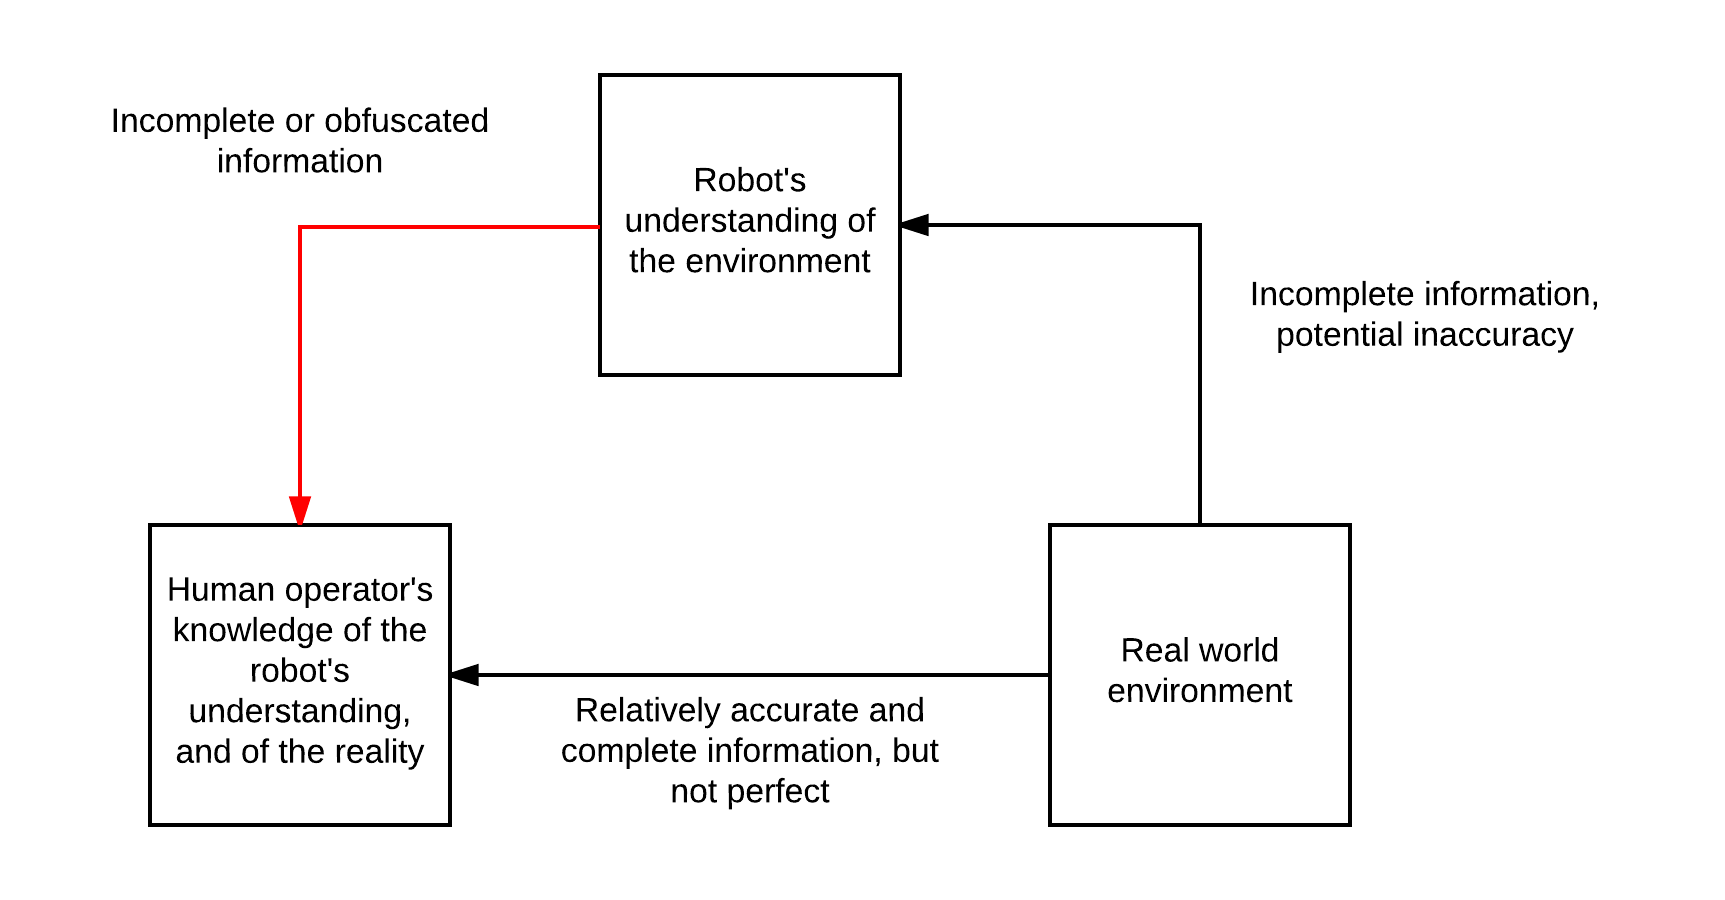
\includegraphics{Figures/RobotDebuggingInformationAbstraction.png}
	\decoRule
	\caption[Debugging Information]{Layers of information abstraction in robotics debugging.}
	\label{fig:DebuggingInformation}
\end{figure}

%----------------------------------------------------------------------------------------

\section{Project Concept} \label{ProjectConcept}
This project focuses on mitigating the problems discussed in the previous section, thus improving the timeliness with which bugs identified in a swarm robotics system can be located and fixed, by improving the operator's access to system information. This means collecting information from multiple sources and presenting it all in one place, in a human readable manner, in real time. The information sources to be used include the individual robots themselves, as well as a live camera feed of the robots' environment.

This project attempts to achieve this by creating a software application and associated wireless data transaction format to present a user with a single, coherent, and highly readable interface through which they can view relevant information about the swarm and it's constituent robots in real time. This includes the use of a video based tracking system to monitor robot positions, and provide the user with a view of the robots' environment. This can then be augmented with graphical representations of relevant elements of the data retrieved from the robots, such as sensor readings. The robots will communicate data to the computer running the application wirelessly. The wireless protocol to be used initially will be WiFi, with Bluetooth to be considered as a possible extension. The initial target robot platform is the widely used \textit{e-puck} robot [!!EPUCK REF!!], equipped with a Linux extension board and WiFi adapter, hence the choice of WiFi as the first wireless protocol to support. The e-puck platform is discussed in greater detail in section . The diagram in Figure  gives a logical representation of the proposed system architecture, in terms of its components, including the e-puck robots, tracking camera, and the application's host computer. This report describes the design, implementation and testing of this system, and includes details of the steps undertaken to evaluate its effectiveness. Some portions of this report appeared previously in a similar form in an \textit{Initial Report}, and are included here for completeness, with minor alterations.

\begin{figure}
	\begin{center}
	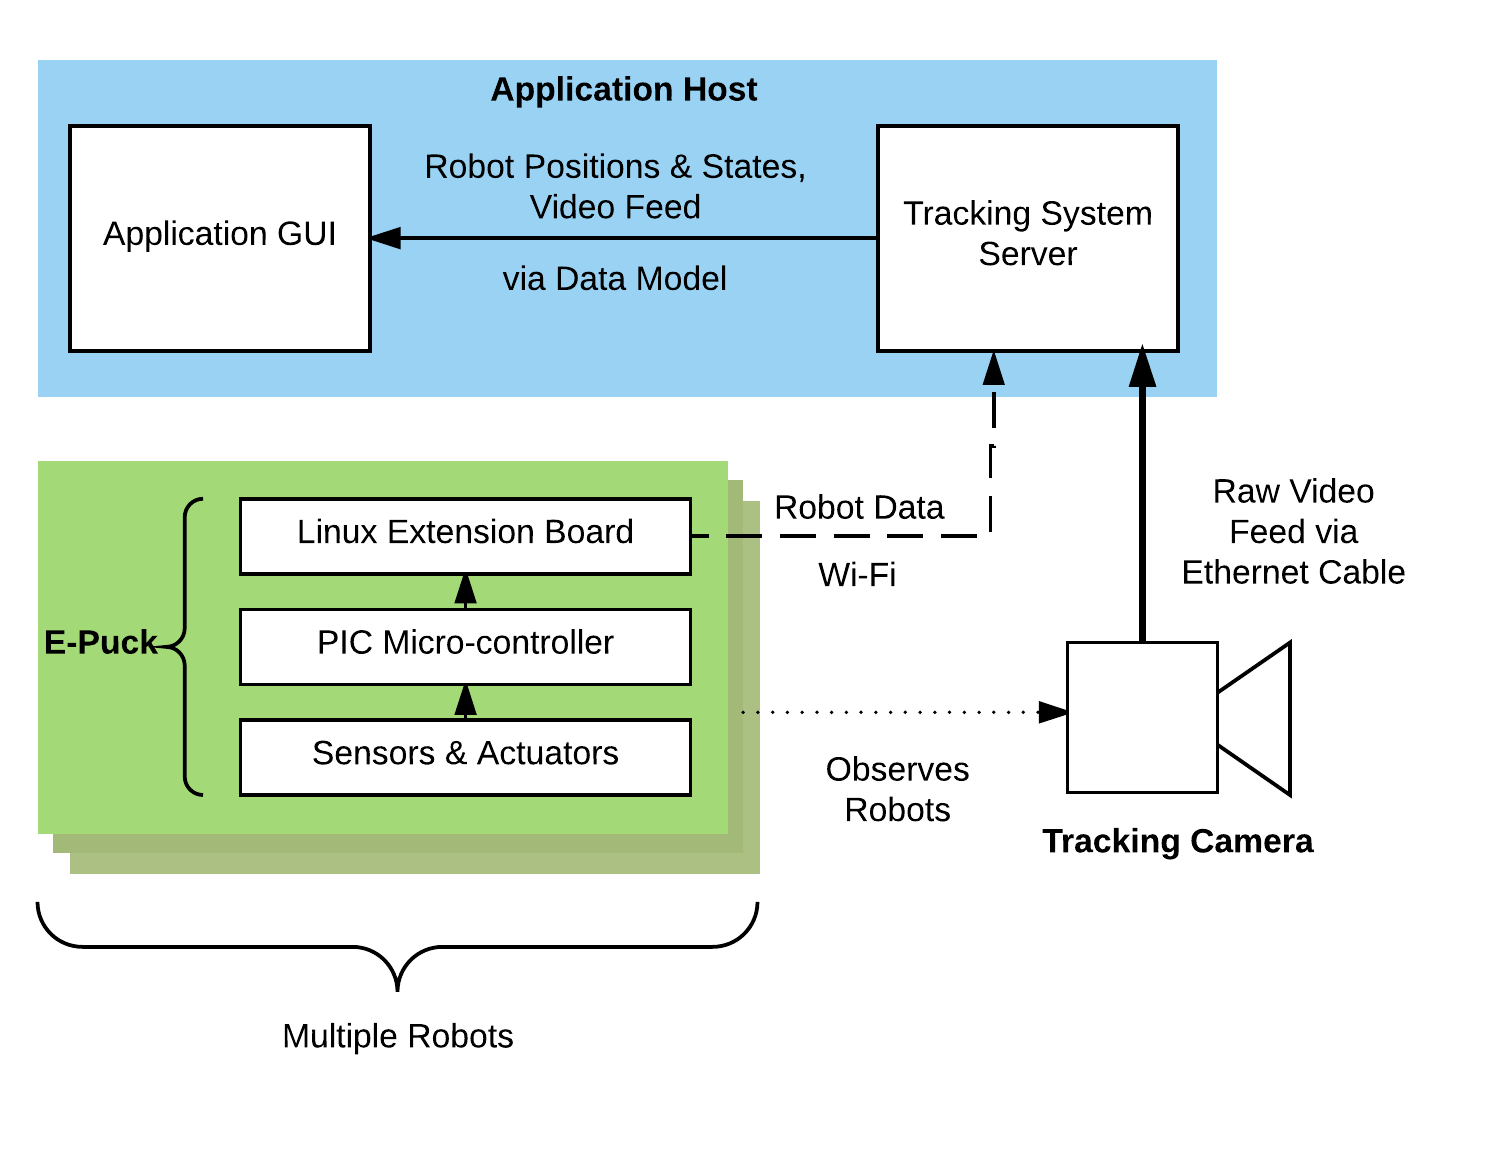
\includegraphics[scale=0.8]{SystemArchitecture.png}
	\decoRule
	\caption{The proposed system architecture.}
	\label{fig:SystemArchitecture}
	\end{center}
\end{figure}

%----------------------------------------------------------------------------------------

\section{Aim and Objectives}
Given the descriptions of the project context and concept in sections \ref{ProjectContext} and \ref{ProjectConcept}, the project aim can be formalised, and a set of objectives determined. This project aims to understand the needs of a swarm robotics researcher or system developer when attempting to debug their system, and create a computer application which allows a user to monitor the state and behaviour of a robot swarm system in real time, thus improving the ease and efficiency of this debugging process. The objectives required to achieve this aim are as follows:

\begin{itemize}
	\item Utilize existing fiducial marker based tracking technology to track the position of individual robots within a swarm over time.
	\item Develop code for presenting the user with a live video feed of a robot swarm, augmented with relevant and spatially situated information relating to the robots, using the data obtained from the tracking system.
	\item Develop code to allow multiple robots to communicate information regarding their internal state, sensor readings and decision making to the main application wirelessly via a network.
	\item Develop a data model that allows the application to store the information it receives from the robots, and update it as new information arrives.
	\item Develop code to ascertain higher level data related to the robots, such as recent movement history or state trasition history, and add this data to the model.
	\item Design and implement a user interface which presents the data model to the user in a human readable manner, and performs data fusion on the information provided by the robots and the tracking information.
	\item Develop the user interface in such a way as to allow the user to filter out information that is not currently relevant, and to contrast and compare information related to specific robots.
	\item Design and implement the system in a modular way so as to allow for relatively simple integration with other swarm robotic platforms and tracking systems in future extensions.
\end{itemize}

%----------------------------------------------------------------------------------------

\section{Functional Specification}
When developing software of any kind it is common practice to define a software specification prior to starting development. This specification describes the functionality required in the software in order for it to satisfy its purpose. The specification presented here is separated into core and secondary requirements. Core requirements are considered essential to the satisfactory delivery of the software. Secondary requirements will be satisfied where possible, given the time constraints of the project.

\textbf{Core Requirements:}
\begin{enumerate}
	\item Must be comprised of a PC application.
	\item Must be capable of receiving data related to the state of multiple robots.
	\item Must be capable of receiving positional data for the same set of robots.
	\item Must be capable of receiving a live video feed of the robots in their environment.
	\item Must collate received data and present it to the user in a combined graphical form.
	\item Must present auxiliary, non-spatial data to the user in textual or other forms.
	\item Must update in approximately real time.
	\item Must at minimum support the e-puck robot platform.
\end{enumerate}

\textbf{Secondary Requirements:}
\begin{enumerate}
	\item Should use a modularised structure.
	\item Should exchange data between the robot platform and the application using a platform-agnostic, extensible protocol.
	\item Should provide a basis for interoperability with a number of robotics platforms.
	\item Should allow the user to configure the displayed data.
	\item Should employ a model-view-controller (MVC) software architecture.
	\item Could provide the user with ways to configure and display custom data types.
	\item Could allow the user to compare data on two or more specific individual robots.
	\item Could calculate and display swarm-level meta-data and statistics.
	\item Could generate log files of robot activity over a user defined period.
\end{enumerate}

%----------------------------------------------------------------------------------------

\section{Report Structure}
This report begins with a survey of the existing literature relevant to the project topic. Individual pieces of research and writing with relevance to some area of the project are highlighted. The project plan is then outlined, with details of the tasks to be undertaken and the time allocated for each, as well as the risk assessment made at the start of the project. This is followed by a short statement on ethics. The hardware to be used in the project is then examined in detail, with information about the target robot platform, the e-puck, and details of the camera and tracking system. The results of an initial survey of some potential users of the system is then presented, and the effect of these results on the implementation are summarised. The design process is then described in detail, including both the structural design of the software architecture and the design of the user interface. The next section gives details of the implementation of the software. This is followed by a description of the testing processes used to verify the software and the results, and details of how the system's effectiveness was evaluated. The penultimate section focuses on possible future work that could be carried out to improve the system. Finally the conclusion looks at the system as a whole, discusses its effectiveness, shortcomings, and its place in the wider field of swarm robotics.